%This file will discuss the design process & additional routes that could have been taken
%This file should be included in doc using \input{file}

\section{Methods}


\subsection{Simulations}

In order to begin pursuing the simulation, problem areas were first identified.  This is to say, the investigation or creation of blocks that we had no experience with.  The PID and other control blocks used in the simulation we were already accustomed to.  Other blocks such as addition, gain, (de)multiplexers, and other common blocks we were also familiar with.  The solutions to these problem areas, as well as the overall design of the simulation is discussed in section \ref{proposed:simulations}.  The problem areas that we identified were as follows:

\begin{itemize}
	\item HID Input
	\item Physical simulation
	\item Real-time rendering
\end{itemize}

The investigation into these issues would first begin by searching for existing blocks or packages within SimuLink.  In the absence of already existing solutions, useful packages would be identified.  Any packages or blocks that could be used as tools to build the desired effect.  Subsequently, the amount of effort to build the result into the simulation using these packages would then be evaluated.  However, in the progression of the simulation, the majority of the tools (as discussed in section \ref{proposed:simulations}) were easily used to implement the problem areas.

\subsection{Physical Implementation}

The physical implementation of the system began with determining a method to interface a controller input with a base station host. To do this, research of available python libraries was performed. It was determined quickly that the most effective route would be to use Python's Pygame library which analyses a bluetooth or usb connected device and determines the types of control inputs applicable for the device. Initially, a PS4 bluetooth connected controller was successfully utilized, receiving all axis and button inputs through the Python interface. 

The next challenge of the physical implementation was to determine the best method of Wi-Fi communication. It was determined that Python's socket library would be best suited, and a Raspberry Pi 3 with a Wi-Fi module available would act as the server in the server, client architecture. A preliminary communication server client script set was written and tested successfully between the base station laptop and the Raspberry Pi server host. 

For the controller host, two possible solutions were considered. Utilizing an Arduino micro-controller as a permanent host of the control loop, communicating with the Raspberry Pi to receive control input data or using the Raspberry Pi for both communication and the controller. Using Arduino would provide a dedicated control loop and an intuitive interface to prototype with. The Raspberry Pi is capable of running the control loop, but issues with regards to a real time operating system were anticipated. Using an Arduino would require more mounting space on the drone as well as another communication channel between the RPi and Arduino to troubleshoot. Many other controllers could have been considered but both RPi and Arduino are owned by group members.

The controller required input from a 10 degree of freedom inertial measurement unit to calculate yaw, pitch, roll and altitude to poll and compare to the control set points. Eventually, alternative methods of calculating altitude were considered and discussed. The methods included infra-red distance sensing, ultrasonic sensing, multiple barometers coupled with Kalman filters, or a barometer accelerometer coupling. PI and PID loops were researched to be implemented on the controller. Several additional filtering techniques were considered for altitude measurement, including moving average filtering, averaging filtering and Kalman filtering with a feedback loop for comparison.

Communications between the RPi and the Arduino were researched, using the interface to interface bus or the serial communication channel were both considered. The data was required to be transmitted as single bytes, thus an algorithm to convert received bytes into floating point values needed research and development.

From a technical background perspective, research regarding the Python language and Python's available libraries was required. Server to client interfacing is also required technical background. Previous knowledge of the Python language assisted in directing the research and development flow throughout the project. PI and PID control loop knowledge was required and research time was used to learn filtering processes, Arduino library development, miscellaneous communication algorithms and utilization of the Adafruit 10 DOF IMU.



\subsection{Graphical User Interface}
\subsubsection{Framework Selection}

There is a multitude of frameworks available for graphical user interface development so in order to narrow down the choices the following restrictions were placed: 
\begin{itemize}
	\item Must function on Windows, Mac OS and UNIX environments
	\item Have the ability to display live plots
	\item Be compatibile with the physical controller initialization software
	\item Have well documented libraries for ease of development 
\end{itemize}
With these restrictions placed and further research into various frameworks the selections narrowed down to Qt and PyQt5. Each of these use the Qt framework which is regarded as a reliable, cross-platform GUI development software with extremely well documented libraries which met the major requirements. Although both Qt and PyQt5 use the same framework there are a few key differences. 

The most notable difference at first glance is that the two use different languages, Qt uses C++ where PyQt5 uses Python but the biggest difference is in the design suites. When developing using Qt you're able to use the QtCreator design suite which allows the user to design the look of the GUI using click and drag widgets, code the functionality of the widgets then simply compile all within the design suite. When using PyQt5 there isn't a complete design suite, instead the user must design the user interface using QtDesigner and then import the GUI file into the Python script, from here the widgets are coded is relatively the same other than the obvious differences between C++ and Python. To finalize the decision on which framework to use two basic GUI's with the same functionality were developed using Qt and then PyQt5. 

The basic GUI was to have the ability to call the PS4 controller initialization script and manipulate the axis settings. Because the initialization script was written in Python it was very difficult and time consuming to do this using the C++ version of Qt compared to using PyQt5 where all that had to be done was import the script. Because each of the scripts that the GUI needs to call are written using Python it was decided to carry on using PyQt5. On top of the ease of importing the scripts using PyQt5 it also allows us to use the vast amount of Python libraries that are available. With the development framework decision made it was time use QtDesigner to design the layout of the GUI that will be intuitive for the end user.

\subsubsection{GUI Layout}  
The layout of a GUI can make or break the end users experience, a clunky non-intuitive GUI will undoubtably cause the end user an unneeded headache. For this reason, a prototype of a graphical user interface was developed and sent to our client to get an idea of what he would be comfortable with and then this prototype was optimized based on his comments. The optimized layout was presented to each of the group members and a consensus was made to move forward using the new layout as it provides all of the required functionality in a clean manner. 

A snapshot of the original prototype layout can be viewed in APPENDIX X, and the final layout can be viewed in the figures below. The purpose and functionality of the widgets will be discussed in the following section. With the layout of the GUI decided on it was time to begin developing the functionality of the widgets.
\begin{figure}[H]
	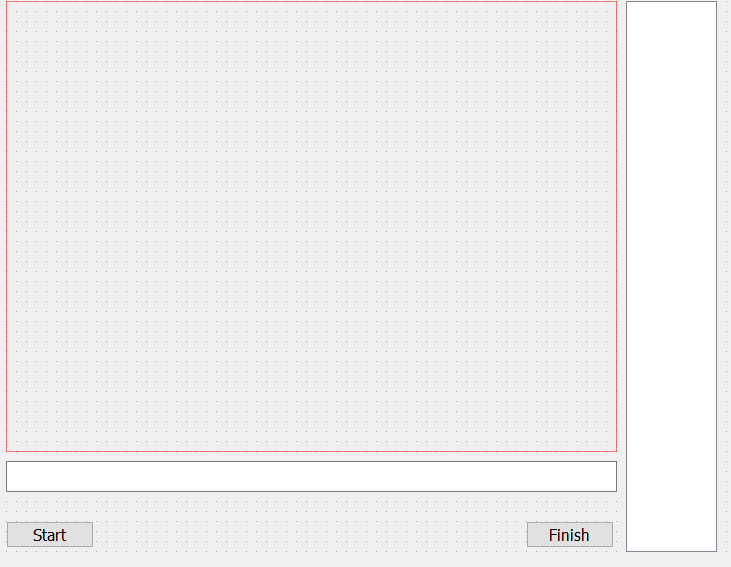
\includegraphics[width=\linewidth]{Final_GUI_HOME.png}
	\caption{Final GUI Home Page}
	\label{fig:GUIHome}
\end{figure}
\begin{figure}[H]
	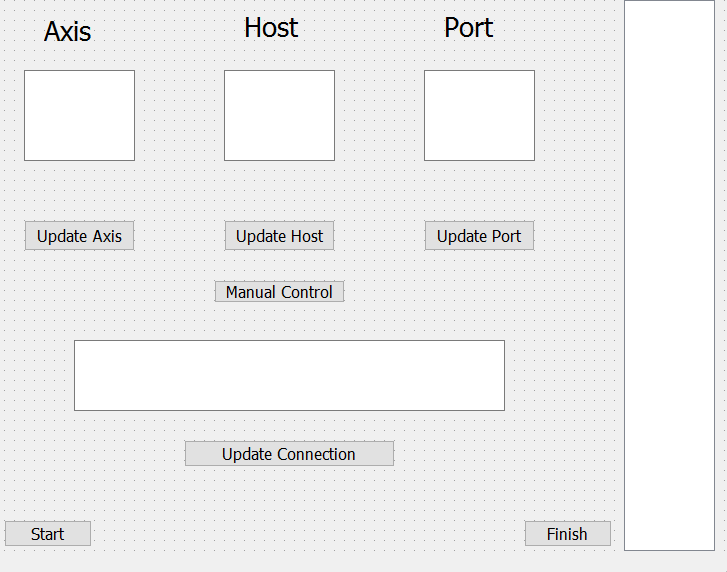
\includegraphics[width=\linewidth]{Final_GUI_CTRL.png}
	\caption{Final GUI Controller and Network Settings page}
	\label{fig:GUICtrl}
\end{figure}

\subsubsection{Widgets}





